\documentclass[fleqn,a4paper]{article}
% code <- needs to be first, only use when adding code blocks
% \usepackage{minted}
% basic settings
\usepackage[ngerman]{babel}
\usepackage[utf8]{inputenc}
\usepackage[babel,german=quotes]{csquotes}
\usepackage[T1]{fontenc}
% layout
\usepackage{conf/arxiv-paper}
% package tools
\usepackage{etoolbox}
\usepackage{xpatch}

% style
\usepackage{newpxtext,newpxmath}
\usepackage[final]{microtype}
\usepackage{hyperref}
\usepackage{url}
\usepackage{color}
\usepackage{booktabs}
\usepackage{bookmark}

% tables
\usepackage{tabularx}

% figures
\usepackage{subfigure}
\usepackage{graphicx}
\usepackage{float}
\graphicspath{{./res/}}

% lists
\usepackage{enumitem}
\setlist[itemize]{leftmargin=*}

% references
\usepackage[
  backend=biber,
  style=numeric-comp,
  citestyle=numeric
]{biblatex}
\bibliography{bib/ref}
% allow an additional line-breaking pass by given size
\emergencystretch=1em

% Math
\usepackage{ntheorem}
\usepackage{dsfont}
\usepackage{nicefrac}
\setlength{\mathindent}{3em}
\usepackage{mathtools}

% lists
\setenumerate{label=(\arabic*),itemsep=3pt,topsep=3pt}

% indentions
\newlength\tindent
\setlength{\tindent}{\parindent}
\setlength{\parindent}{0pt}

% arxiv settings
\setcounter{tocdepth}{2}
\renewcommand\UrlFont{\color{blue}\rmfamily}

% commands
\DeclarePairedDelimiter{\abs}{\lvert}{\rvert}
\newcommand{\N}{\mathds{N}}
\newcommand{\R}{\mathds{R}}
\newcommand{\E}{\mathbf{E}}
\renewcommand{\L}{\mathcal{L}}

%%%                  %%%
% document information %
%%%                  %%%

\title{Business Intelligence: Customer Analytics}
\author
  {\textbf{Paula Möller}\\
  Fachbereich Informatik\\
  Hochschule Darmstadt
  \and
  \textbf{Maximilian Neudert}\\
  Fachbereich Informatik\\
  Hochschule Darmstadt
}

%%%      %%%
% document %
%%%       %%

\begin{document}
% title
\maketitle

% abstract
\begin{abstract}
Diese Arbeit beschäftigt sich mit der Customer Analytics zu dem Zweck der Intensivierung der Kundennähe. Ziel war es, einen Überblick über das komplexe Feld der Customer Analytics zu geben und durch die Veranschaulichung an einem Beispiel die Relevanz und Techniken für die Durchführung in der Unternehmenspraxis exemplarisch aufzuzeigen.
Das dazu durchgeführte Clustering auf einem Datensatz aus dem Einzelhandels-Umfeld kann als ein prototypisches Vorgehen betrachtet werden, welches aufgrund der exemplarischen Ausführung keine direkt für die operative Umsetzung relevanten Ergebnisse liefert, aber mögliche Implementationsstrategien und Erweiterungen für eine Anwendung in Business Intelligence Systemen aufzeigt.
Vielmehr kann diese Arbeit somit als ein Einstieg in das Themenfeld der Customer Analytics im Business Intelligence Kontext gesehen werden.
% keywords
\keywords{Data Science \and Business Intelligence \and Customer Analytics \and CRM \and Data Mining}
\end{abstract}

% toc
\clearpage
\tableofcontents

% content
\clearpage
\section{Einleitung}
\label{sec:einleitung}

Bereits 1993 konnte in einer Studie von Treacy und Wiersema \cite{wiersema1993} die Relevanz von Customer Analytics gezeigt werden. Ziel dieser dreijährigen und 80 Unternehmen umfassenden Studie war, Merkmale von marktführenden Unternehmen zu identifizieren, die für deren marktbeherrschende Position ausschlaggebend waren. Dabei fand eine Gegenüberstellung von sog. \textquote{value propositions} (den Versprechen der Unternehmen gegenüber den Kunden), mit den jeweiligen internen Strategien, Abläufen und Strukturen statt. Treacy und Wiersema konnten drei dominante Strategien aufzeigen (die sogenannten „value strategies“). Neben den Strategien der operationalen Exzellenz und der Produktführerschaft wurde die Kundennähe als entscheidender Wettbewerbsvorteil identifiziert.

Die operationale Exzellenz wird als eine solche Unternehmensführung bezeichnet, die als „dynamische Fähigkeit zur Rea­lisierung von effektiven und effizienten Kernprozessen der Wertschöpfungskette“ \cite{gleich2008} der Optimierung des Verhältnisses von Qualität und Preis dient. Die Produktführerschaft kann unterdessen als das für den Kunden beste Produkt verstanden werden.

Für eine strategische Ausrichtung im Sinne der Kundennähe muss das Unternehmen jedoch nicht das günstigste oder innovativste Produkt führen, sondern dem Kunden die beste individuell zugeschnittene Lösung bieten.

Die Kundennähe konnte damit als einer von drei entscheidenden Faktoren aufgezeigt werden. Und obwohl ein Fazit der Studie war, dass ein Unternehmen sich in einer der drei Strategien profilieren sollte (während die anderen beiden nur auf einem dem Wettbewerb angemessenen Niveau gehalten werden müssen), war trotzdem eine Veränderung der Unternehmensstrategien von zuvor stark produkt-dominierter Auslegung zu einer kundenzentrierten Sichtweise zu beobachten. Bereits 2010 konnte in einer Studie des IBM Institute for Business Value \cite{ibm2010} die Kundennähe als „number-one priority“ führender Unternehmen identifiziert werden.

Diese Entwicklung wird zusätzlich durch Zeiten umkämpfter und komplexer Märkte verschärft, auf denen Kunden nach zunehmend individuelleren Lösungen verlangen. Die notwendige Veränderung in der Unternehmensstrategie kann nur durch eine Fokussierung auf die Kundenbedürfnisse erreicht werden.

Damit ist ebenfalls eine Veränderung der Marketingmaßnahmen hin zu stärkerer Service- und Beziehungsorientierung zu beobachten, die wiederum zu einer Verschmelzung von zuvor getrennt gehaltenen Unternehmensbereichen führt \cite{olivarogelio2003} und grundlegende Veränderungen der bisherigen Unternehmensstruktur erfordert.

Durch die Erforschung der Kundenperspektive im Sinne der Customer Analytics wird diese Entwicklung überhaupt erst ermöglicht.
\section{Begriffsbestimmung und Einordnung}
\label{sec:begriffsbestimmung_einordnung}

\subsection{Bezug zu der Business Intelligence}
Die Customer Analytics ist ein Teilgebiet der Business Intelligence, die wiederum als die „Extraktion und Auswertung der unternehmensweit vorhandenen Daten und deren Umwandlung in für die Entscheider relevante Informationen“ \cite[S. 6]{hannig2002} durch verschiedene Softwarewerkzeuge bezeichnet werden kann.
Der Einsatz von Werkzeugen und Anwendungen der Business Intelligence soll zu einer „besseren Einsicht in das eigene Geschäft und damit zu einem besseren Verständnis in die Mechanismen der relevanten Wirkungsketten führen“ \cite[S. 32]{hannig2002}.

Dabei kommt dem internen Wissensmanagement als Voraussetzung für erfolgreichen Einsatz der Softwarewerkzeuge große Bedeutung zu. Dieses gliedert sich in die Teilbereiche der „Gewinnung von Wissen aus allen verfügbaren Quellen, die Strukturierung, Aufbereitung und Speicherung des generierten Wissens und die bedarfsgerechte Zurverfügungstellung des Wissens“ \cite[S. 16]{hannig2002}.
Je nach Perspektive umfasst der Begriff Business Intelligence unterschiedliche große Bereiche. Eine sehr weite Auslegung würde alle Tools umfassen, mittels denen operatives Datenmaterial gewonnen und ausgewertet werden kann.
Damit würden auch die Datenquellen selbst zu der Business Intelligence gezählt werden. Eine etwas engere Definition über ein analyseorientiertes Verständnis schließt diese aus, umfasst jedoch noch weitere Maßnahmen über Data Mining, Kennzahlen oder analytisches Customer Relationship Management (CRM), die in der engsten definitorischen Sichtweise nicht mehr beinhaltet sein würden.\cite{hannig2002}

\subsection{Konzeptualisierung und Definition}

Der Begriff Customer Analytics findet keine einheitliche Definition in der Literatur. Vielmehr wird sich diesem auf Basis verschiedener Kennzahlen angenähert, die sich wiederum auf Teilgebiete der Customer Analytics beziehen.

In diesem Abschnitt wird daher zunächst eine konzeptionelle Grundlage durch die Theorie informationeller Mehrwerte gegeben, im Anschluss daran eine Arbeitsdefinition aufgestellt und nachfolgend einige Kennzahlen vorgestellt, die eine Abgrenzung und ein besseres Verständnis des Themenbereiches ermöglichen.

\subsubsection{Die Theorie informationeller Mehrwerte}
Als Grundlage der Customer Analytics wird auf die Theorie informationeller Mehrwerte \cite{kuhlen1995} verwiesen. Kuhlen versteht als informationellen Mehrwert einen über den Grundwert hinaus gehenden Zusatzwert, der aber auch erst kundenseitig als solcher empfunden werden muss, um als ein solcher Mehrwert bezeichnet werden zu können.

Um eine Mehrwertleistung bieten zu können, braucht es demnach Wissensbestände, aus denen Informationen über Wünsche und Ansprüche der Nutzer bzw. Kunden abgeleitet werden können.

\subsubsection{Definition}
Der dieser Arbeit zugrunde liegende Begriff der Customer Analytics wird damit ausgehend von der Theorie informationeller Mehrwerte als ein Prozess verstanden, bei dem aus der Analyse der dem Unternehmen vorliegenden Kundendaten (neue) Erkenntnisse gewonnen werden, um das operationale und strategische Management daraufhin auszurichten. \cite{kumar2018}

Customer Analytics dient also der Erforschung der Kundengruppen und deren Bedürfnissen bzw. deren Zufriedenheit. Dafür werden Kundengruppen auf Basis ihres Verhaltens segmentiert, um zukünftiges Verhalten vorherzusagen oder Trends zu erkennen oder um Marketing- bzw. Vertriebsaktivitäten gezielt auf Kundengruppen ausrichten zu können. \cite{gartner2020}

Je nach Verständnis der Business Intelligence können Maßnahmen der Customer Analytics nur in den analyse-orientierten Teil der Business Intelligence eingeordnet werden und gehören damit nicht zu den Kernelementen der Business Intelligence.

\subsection{Praxisorientierte Anwendung der Customer Analytics}
Für die Erzeugung eines informationellen Mehrwertes im wirtschaftlichen Umfeld müssen auch in der Customer Analytics zunächst Kundeninteressen bekannt sein. Die dieser Ermittlung zugrunde liegenden Daten sind aus einer Vielzahl möglicher Interaktionen mit dem Kunden entstanden. Kunden können dabei Individuen, aber auch Gruppen oder Organisationen sein. Informationen über diese werden in einem Datenbanksystem abgelegt, welches gleichzeitig das CRM ermöglicht, auf das in nachfolgenden Abschnitten vertieft eingegangen wird.

Die anwendungsorientierte Customer Analytics beruht also zum einen auf den Datenbeständen über die Kunden aus den internen Systemen, welche sich in einem stetigen Veränderungsprozess befinden. Daher müssen diese Daten laufend angepasst bzw. aktualisiert werden, um verlässliche Aussagen treffen und daraufhin die Unternehmensstrategie auslegen zu können. Im digitalen Kontext können zum anderen als weitere Datenquelle Transaktionsdaten bzw. Daten aus dem Tracking des Navigationsverhaltens der Nutzer/Kunden verwendet werden, die durch Data Mining Techniken ausgewertet werden. Die Auswertung der anfallenden Datenmengen (Big Data) werden also im Zuge der der Customer Analytics ausgewertet. Daher wird in diesem Zusammenhang zunehmend der Begriff „Smart Data“ verwendet.

Aus dem Vorliegen von Big Data wird zugleich eine der beiden Herausforderungen der Customer Analytics \cite{choudhury2010} deutlich. Dem Unternehmen liegen nahezu unbegrenzte Möglichkeiten von Metriken vor, um eine Analyse durchzuführen. Choudhury et al. \cite{choudhury2010} bezeichnen dies als das „relevance“ Phänomen. Als eine weitere Schwierigkeit der Customer Analytics bezeichnen sie die „inference“. Diese resultiert aus dem Problem, relevante Komponenten für die Analyse nicht direkt aus dem existierenden Datenbestand entnehmen zu können, sondern aus weiteren Maßnahmen zu erschließen.

\subsection{Verwendung von Kennzahlen in der Customer Analytics}
Für eine Einschätzung und Vergleichsmöglichkeit individueller Kunden oder Kundengruppen werden in der Praxis häufig Kennzahlen der Customer Analytics eingeführt.

Diese Key Perfomance Indicators (KPIs) umfassen Dimensionen, wie den Umsatz, die Zeit zwischen Transaktionen, den Anteil der gekauften Produktkategorien, die Preissensitivität uvm. \cite{grigsby2016}. Auch hier werden die Ergebnisse aus dem Kundenverhalten abgeleitet.

Neben der Segmentierung von Kundengruppen bieten die Customer Lifetime Value (CLV), die Customer Profitability (CP) oder die Recency-Frequency-Monetary Methode (RFM-Methode) weitere Bewertungsmöglichkeiten. Die ersten beiden KPIs sind zur Messung von Unterschieden der Konsumenten geeignet \cite{pfeifer2005} und ergeben ein wertbasiertes Urteil über den jeweiligen Kunden.
Der Unterschied besteht darin, dass die CLV ein Urteil über Deckungsbeitrag eines Kunden zu einem gegebenen Zeitpunkt macht, wobei in der CP das Kosten-Nutzen-Verhältnis eines Kunden betrachtet wird.

Die RFM-Methode \cite{fader2004} wiederum kombiniert drei Faktoren: Recency \textit{(wann hat der Kunde zuletzt eingekauft?)}, Frequency \textit{(wie oft hat ein Kauf stattgefunden?)} und Monetary Value \textit{(wie viel Geld hat der Kunde ausgegeben?)}.

Diese wertbasierten Kundenklassifikationen lassen sich kombinieren \cite{fader2004}.
Aufgrund ihrer geringen Komplexität werden diese KPIs, insbesondere die RFM Methode, gerne in der alltäglichen Marketing-Praxis verwendet. Durch komplexere Techniken der Customer Analytics lassen sich jedoch weitere Unternehmensziele operationalisieren.
\section{Ziele der Customer Analytics}
\label{sec:ziele}

Durch ein tieferes Kundenverständnis können verschiedene direkt auf den Kunden ausgerichtete Disziplinen verbessert werden, dazu zählen Produkte und Services des Unternehmens, sowie das Marketing und ein verbessertes CRM. Somit lassen sich durch Customer Analytics ebenso Teilgebiete der „value strategies“ behandeln.

\subsection{Produkt-/Service-orientierte Optimierung}
Aus Erkenntnissen über Kundenbedürfnisse oder die Zufriedenheit der Kunden können Veränderungen von Produkten und Services bis hin zu vollständigen Prozessen des Unternehmens vorgenommen werden. Für eine Verbesserung der operationalen Exzellenz bzw. der Produktmarktführerschaft im Sinne der „value strategies“ muss ggf. ebenso die Unternehmensstrategie angepasst werden. Alle Prozesse sollten von Beginn an auf den Kunden und dessen möglicherweise veränderte oder individuelle Interessen angepasst sein.
Dies führt ebenfalls zu der Notwendigkeit der Orientierung aller Mitarbeiter des Unternehmens an den Kundenbedürfnissen. \cite{habryn2012}

Durch dabei auftretende Veränderungen und die bereits thematisierte Aufweichung der bisherigen Unternehmensbereiche, müssen auch Mitarbeiter funktionsübergreifend tätig sein.
Damit werden beispielsweise Mitarbeiter, die bisher im Verkauf tätig waren, zu Beratern in Fragen oder Problemen in Zusammenhang mit den Produkten.

\subsection{Operationale Exzellenz im Marketing}
Das Marketing wird durch anfangs geschilderte Bedingungen auf den Märkten zunehmend komplexer und (kosten-)aufwändiger. Aus den Erkenntnissen der Customer Analytics in Verbindung mit den Möglichkeiten der Digitalisierung (z.B. im Sinne direkter Kontaktaufnahme) können Werbemaßnahmen jedoch gezielter ausgeführt werden. Dies ermöglicht den Einsatz personalisierter Werbung bzw. Werbung für bestimmte Kundengruppen (welche bspw. aus einer Segmentierung resultieren). Damit kann zugleich die Effizienz der Werbemaßnahmen gesteigert werden.

\subsection{Kundennähe durch intensiviertes CRM}

In der Studie von Reichheld und Dawkins \cite{reichheld1990}, die eine Vielzahl von Geschäftsbereichen umfasste, konnte gezeigt werden, dass durch eine Erhöhung der Kundenbindung um fünf Prozent der Kunden der gesamte Kundenwert (CLV) um 25 bis 85 Prozent gesteigert werden kann. Techniken der Customer Analytics können also für eine effizientere Gestaltung des CRM genutzt werden. Auf weitere Einzelheiten des CRM in Verbindung mit der Customer Analytics wird in Abschnitt \ref{sec:crm} vertieft eingegangen.

\section{Herausforderungen unterschiedlicher Geschäftsmodelle}
\label{sec:herausforderungen}

Je nach Geschäftsmodell können dem Unternehmen verschiedene Kunden zugeordnet werden.

Im Business-to-Business (B2B) Bereich liegen Geschäftsbeziehungen zwischen zwei oder mehr Unternehmen vor, während im Business-to-Consumer (B2C) Umfeld Geschäftsbeziehungen zwischen dem Unternehmen und Privatpersonen vorliegen. \cite{aichele2016}

\subsection{B2B}
Das B2B Umfeld kennzeichnet sich durch kleinere Kundenbestände, bei denen der Überblick über die bestehenden Kunden besser gewahrt werden kann.

Die Beziehungen zwischen den Geschäftspartnern beruhen stärker auf einer persönlichen Ebene, bei der Maßnahmen der direkten Kontaktaufnahme eine bessere Wirkung erzielen. An der Kaufentscheidung eines Produktes sind dennoch mehr Personen beteiligt, da die direkt mit dem Unternehmen kommunizierende Person häufig nicht selbst für eine Entscheidung über einen Kauf befugt ist \cite{aichele2016}. Aus dieser komplexeren Vertriebssituation und komplexeren Produkten entstehen situationsbedingt unregelmäßigere Käufe. Ohne ein konsequentes CRM können die Kundenbeziehungen nicht aufrecht erhalten werden.

Daher hat sich eine Analyse der Beziehungen der Mitarbeiter des Unternehmens und der Angestellten des Kunden bereits als erfolgreich für die Erklärung des Unternehmenserfolgs gezeigt \cite{gummesson2011}. Diese kann durch Methoden der Netzwerkanalyse ausgeführt werden, die auf personenbezogener Ebene stattfinden und somit ein soziales Netzwerk erstellen \cite{habryn2012}. Besonders entscheidend sind dabei Eigenschaften wie die Größe und die Position der Netzwerke \cite{hutt2006}. Aus analytischer Sicht kann das CRM auf Basis der B2B Umgebung durch weitere KPIs, wie dem CLV ergänzt werden.

Zusammenfassend ist also die Customer Analytics im B2B-Segment weniger entscheidend, da das CRM hauptsächlich zur Unterstützung des operativen Geschäfts benötigt wird.

\subsection{B2C}
Im Vergleich zu dem B2B Kontext ist der Kundenbestand der Unternehmen, die hauptsächlich im B2C Bereich agieren, deutlich umfassender. Kunden sind primär Privatpersonen, die sich in weniger komplexen Entscheidungssituationen über weniger komplexe Produkte befinden. Dennoch bringt auch dieses Geschäftsmodell Schwierigkeiten für die Customer Analytics, denn die Entscheidung wird durch eine Vielzahl nicht kontrollierbarer und nicht vorhersagbarer, zumeist unbekannter Faktoren bestimmt. Dies erschwert die Vorhersagbarkeit des Kundenverhaltens. 

Dennoch kommt hier die Customer Analytics stärker zum Tragen, da aufgrund von massiven, sich schnell verändernden Datenbeständen und vieler paralleler Transaktionen keine rein operative Steuerung aus dem persönlichen Kontakt heraus möglich ist.

Für die Einflussnahme auf eine abgrenzte Gruppe oder einzelne Kunden eignen sich beispielsweise Clustermethoden, die eine individuellere Interaktion mit dem Kunden ermöglichen. Damit werden Daten aus CRM Systemen für die Unterstützung analytischer Auswertungen benötigt und müssen fortschreitend durch Methoden der Customer Analytics ausgewertet werden. \cite{aichele2016}

\section{Customer Relationship Management}
\label{sec:crm}

\subsection{Motivation}

CRM ist die \textquote{Planung, Steuerung und Durchführung aller interaktiven Prozesse mit den Kunden} \cite{crm_gabler2020}, die durch Kundenorientierung und Individualisierung unter Berücksichtigung der CLV der jeweiligen Kunden eine Langfristigkeit der Kundenbeziehungen anstrebt (ebd.).

CRM wird ausdrücklich nicht als zeitlich eng begrenztes Projekt oder als reines IT-Projekt verstanden, sondern als kundenorientierte Unternehmensstrategie, deren Implementierung in einem kontinuierlichen organisatorischen Lernprozess abläuft \cite[S. 47]{grundcrm}.
Vorraussetzung hierfür seien unter anderem eine intensivere IT-Unterstützung durch leistungsfähige CRM-Systeme.
Das Ziel von CRM-Systemen ist es, auf Basis einer Kundendatenbank, Marketing, Vertrieb und Service zu bedienen und eine ganzheitliche Sicht auf einzelne Kunden zu schaffen und damit einen passenden Dialog zu ermöglichen.

Als integrative Aufgabenstellung von CRM-Systemen ergeben sich nach \cite[S. 47]{grundcrm}:
\begin{itemize}
  \item Die Synchronisation und operative Unterstützung der zentralen Customer Touch Points Marketing, Vertrieb und Service,
  \item die Einbindung aller Kommunikationskanäle zwischen Kunde und Unternehmen,
  \item sowie die dazu erforderliche Zusammenführung und Auswertung aller Kundeninformationen.
\end{itemize}

Dies führe zu einer hohen Komplexität von CRM-Systemen, welche sich in operative und analytische CRM unterteilen lässt. \cite{kumar2018}

Im operativen Sinne kann das CRM durch rechnergestützte Verwaltung von statischen Kundendaten und aus Transaktionen resultierenden Kundendaten die Aufrechterhaltung des Kontaktes und vereinfachte Transaktionen unterstützen.

Das analytische CRM wird durch Techniken der Customer Analytics ermöglicht bzw. ist eng mit diesen verbunden. Dabei steht der Erkenntnisgewinn aus den vorliegenden Daten im Vordergrund \cite{kumar2018} und somit den für Business Intelligence relevanten Teil darstellt, wie in Abbildung \ref{fig:crmcomps} illustriert.

\begin{figure}[ht]
  \centering
  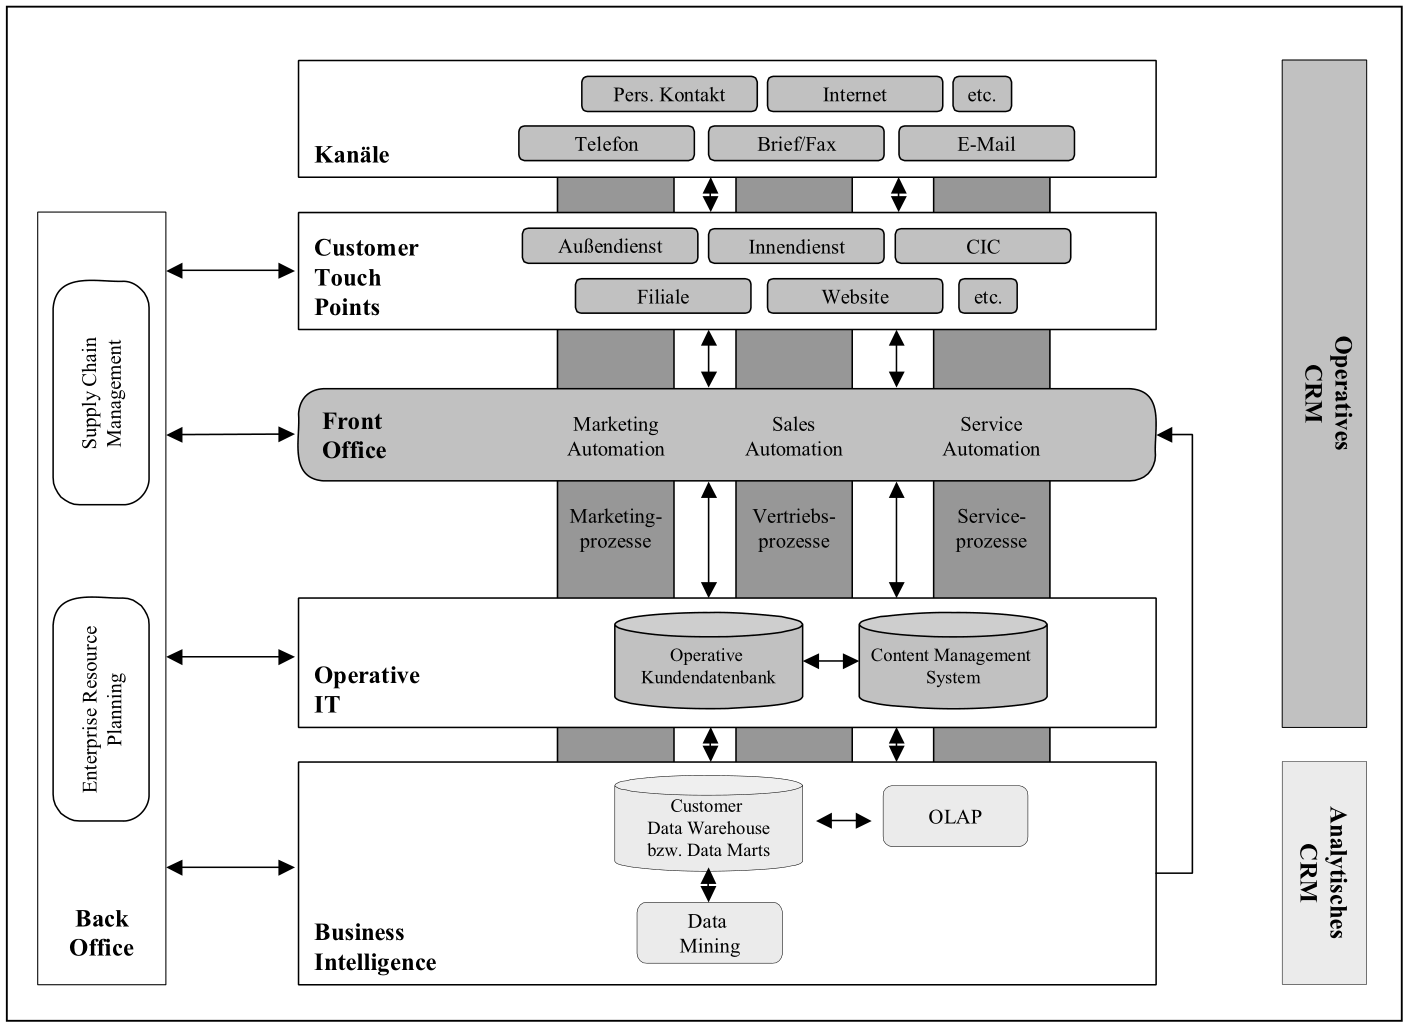
\includegraphics[width=0.9\textwidth]{crmcomps}
  \caption{Komponenten eines CRM-Systems\cite[S. 48]{grundcrm}}
  \label{fig:crmcomps}
\end{figure}

Die für die Business Intelligence relevanten Komponenten lassen sich in OLAP, Data Mining und Customer Data Warehouse bzw. Data Marts einteilen.

\subsection{Data Warehouse und OLAP}

Grundlage für die Differenzierung der Kundenbeziehungen bildet die Zusammenführung aller kundenbezogenen Informationen in einem Customer Data Warehouse, welche eine von der operativen Datenbanken getrennte Analysedatenbank darstellt. \cite[S. 49]{grundcrm}
Man bezeichnet dies auch als Data-Mart, also eine Kopie einer Teilmenge, eines Data Warehouse von in diesem Fall kundenspezifischer Daten. Solche Data-Marts sind üblicherweise hochdimensional und das Finden von in den Daten verborgenen, erfolgsrelevanten Geschäftsinformationen erfordert passende Werkzeuge.
Für diesen Zweck wurde das Konzept des On-Line Analytical Processing (OLAP) entwickelt.
OLAP-Systeme bilden betriebswirtschaftlich relevante Maßgrößen in Form eines multidimensionalen Datenwürfels (Abb. \ref{fig:olap}) ab, dessen Dimensionen betriebswirtschaftlich relevante Gliederungskriterien sind.
Entlang dieser Dimensionen können die betriebswirtschaftlichen Maßzahlen je nach Fragestellung aufgebrochen (Drill down) oder aggregiert (Roll up) werden.
Ergänzend kann der Anwender diesen Würfel drehen und kippen (dice) oder in einzelne \textquote{Scheiben} zerlegen (slice).
\cite[S. 49]{grundcrm}

\begin{figure}[ht]
  \centering
  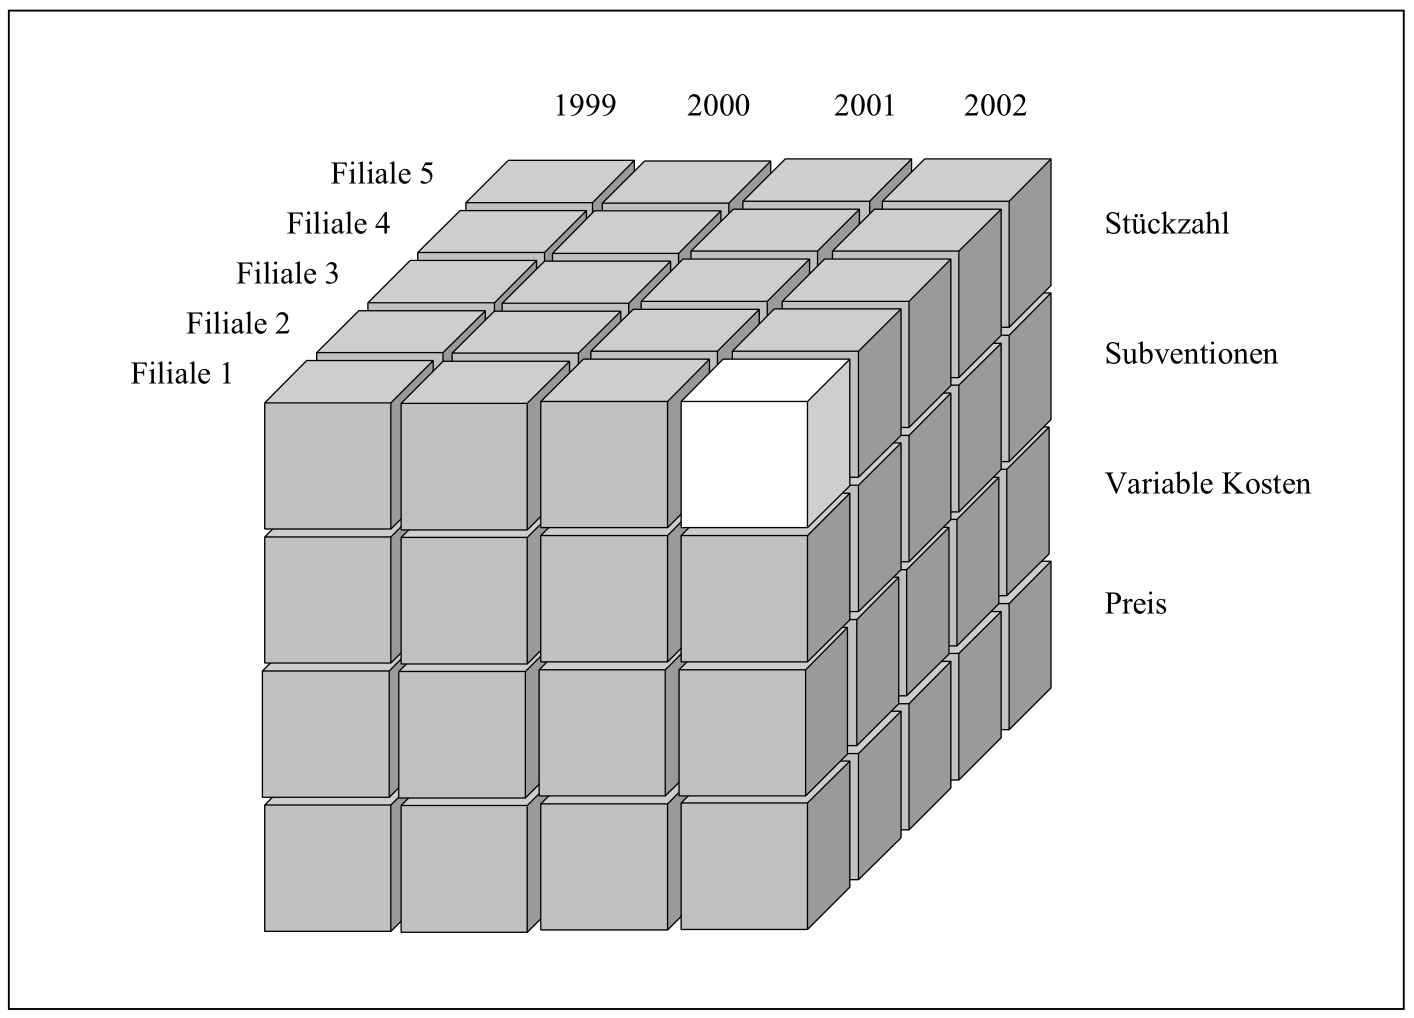
\includegraphics[width=0.9\textwidth]{olap}
  \caption{Beispiel Navigation in einem dreidimensionalen Datenwürfel\cite[S. 50]{grundcrm}}
  \label{fig:olap}
\end{figure}

Zum Erkennen der Zusammenhänge im OLAP-System setzt man Data Mining ein, mit der man die anwenderorientierten Anfragen um automatisierte Suche nach komplexeren Strukturen erweitert.

\subsection{Data Mining Methoden}

Im Rahmen des Data Mining werden Methoden zur Klassifikation, Prognose, Segmentierung und Abhängigkeitsanalyse untersucht und entsprechende Algorithmen entwickelt.

\begin{figure}[ht]
  \centering
  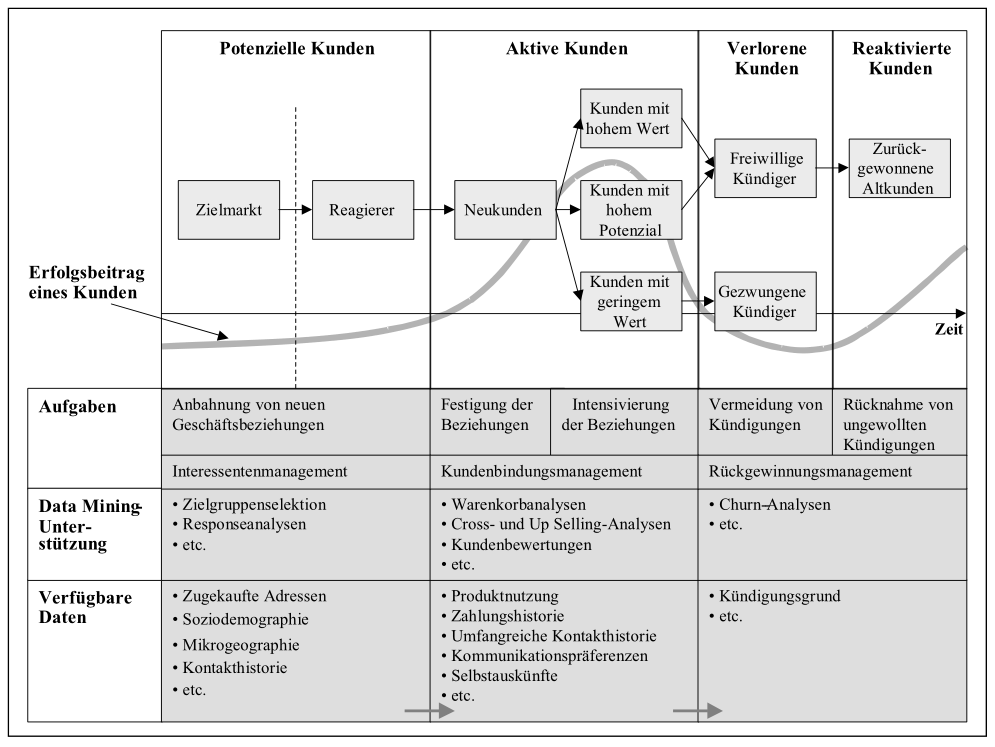
\includegraphics[width=0.9\textwidth]{datamining}
  \caption{Data Mining im Beziehungslebenszyklus\cite[S. 52]{grundcrm}}
  \label{fig:datamining}
\end{figure}

Ein typisches Beispiel der Klassifikation ist die Kündigeranalyse, bei der nach Variablen gesucht wird, die einen möglichst starken Zusammenhang zum Kündigungsverhalten aufweisen und aufgrund derer eine Klassifikation der Kunden möglich wird.
Ein solches Klassifikationsmodell lässt sich auch zur Prognose der Kündigungswahrscheinlichkeit bestehender Kunden einsetzen.
Eine Segmentierung verfolgt das Ziel, Individuen in vorab unbekannte homogene Segmente zusammenzufassen. Hierbei werden durch das Verfahren selbständig Kundensegmente ermittelt, die sich durch ähnliche Merkmalskombinationen auszeichnen.
Ein Beispiel für eine Abhängigkeitsentdeckung ist die Warenkorbanalyse, bei der untersucht wird, welche Produkte typischerweise gemeinsam innerhalb der Käufe eines Kunden auftreten. \cite[S. 51]{grundcrm}

\subsection{Anwendungsbeispiel: CRM im Einzelhandel}

In \cite{biapp} wird ein Beispiel skizziert, in dem ein Unternehmen für eine zielgruppenspezifische Preis- und Rabattpolitik eine Kundenkarte mit einem entsprechenden Bonusprogramm erstellen möchte.

Dazu werden die Verkäufe am Point of Sale (POS) erfasst, in ein Core Data Warehouse geladen und die für die Kampagne relevanten Daten in einem Data Mart zusammengeführt.
Darauf lassen sich dann Analysesysteme für eine Zielgruppenselektion mittels Data Mining Methoden oder klassischen Scorings bzw. o.g. KPIs wie die RFM-Methode \cite{rfmr} aufbauen und für die Zielgruppen die relevantesten Kanäle zum bewerben ermitteln.
Anschließend wird eine Wirkungsanalyse mit dem Ziel der Gewinnung handlungsrelevanter Informationen für den weiteren Verlauf der Kampagne oder zukünfitge Kampagnen durchgeführt. Die Daten aus der Wirkungsanalyse werden dann wieder in den Data Mart eingespeist, um Lernen zu ermöglichen. Dies wird als Closed-loop \cite[S. 223]{biapp} bezeichnet.

Damit erhält man ein Business Intelligence System für die Unterstützung und Steuerung von Entscheidungen, um über CRM den Unternehmenserfolg zu erhöhen. Ein Schema für solch eine Prozesskette ist ist in Abbildung \ref{fig:bieinzel} abgebildet.

Laut \cite[S. 224]{biapp} führte das praktische Umsetzen eines solchen Anwendungsbeispiel zu einer Steigerung der Responsequote um 300\%, während die Anzahl der durchschnittlich angeschriebenen Kunden um 60\% verringert wurde, wodurch das Projekt unternehmensintern als Erfolg gewertet wurde.


\begin{figure}[ht]
  \centering
  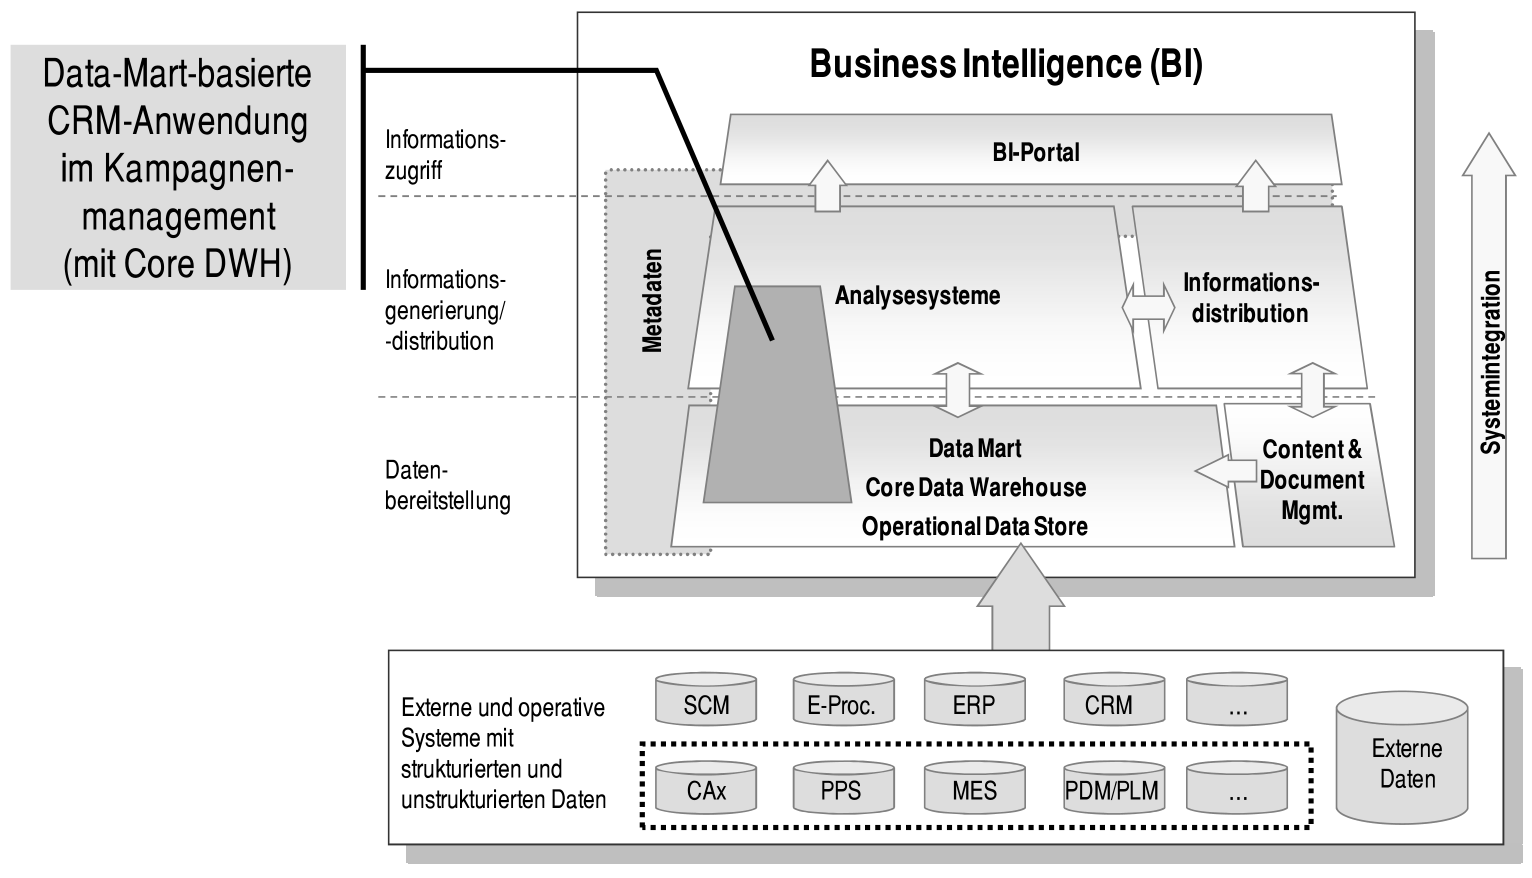
\includegraphics[width=0.9\textwidth]{crmeinzel}
  \caption{CRM im Einzelhandel\cite[S. 220]{biapp}}
  \label{fig:bieinzel}
\end{figure}

\subsection{Anwendungsbeispiel: Supermarket sales (Kaggle)}

In diesem Beispiel wird mögliche Customer Segmentation anhand eines realen Datensatzen aus Kaggle (\url{https://www.kaggle.com/aungpyaeap/supermarket-sales/version/3}) vorgestellt.

Der Datensatz entstammt aus einer Datenerhebung von historischen Verkaufsdaten aus drei Standorten einer Supermarktkette in Myanmar  über drei Monate hinweg.
Jede Zeile ist ein Einkauf und als Feature-Spalten gibt es:

\begin{center}
  \begin{tabular}{l | m{10cm}}
    Invoice id & Computer generated sales slip invoice identification number\\
    Branch & Branch of supercenter (3 branches are available identified by A, B and C).\\
    City & Location of supercenters\\
    Customer type & Type of customers, recorded by Members for customers using member card and Normal for without member card.\\
    Gender & Gender type of customer\\
    Product line & General item categorization groups - Electronic accessories, Fashion accessories, Food and beverages, Health and beauty, Home and lifestyle, Sports and travel\\
    Unit price & Price of each product in \$\\
    Quantity & Number of products purchased by customer\\
    Tax & 5\% tax fee for customer buying\\
    Total & Total price including tax\\
    Date & Date of purchase (Record available from January 2019 to March 2019)\\
    Time & Purchase time (10am to 9pm)\\
    Payment & Payment used by customer for purchase (3 methods are available – Cash, Credit card and Ewallet)\\
    COGS & Cost of goods sold\\
    Gross margin \% & Gross margin percentage\\
    Gross income & Gross income\\
    Rating & Customer stratification rating on their overall shopping experience (On a scale of 1 to 10)
  \end{tabular}
\end{center}

Wie in den Herausforderungen der Customer Analytics aufgezeigt, sind nicht alle erfassten Daten bzw. Features für die Analyse relevant. Daher wurde eine Bereingung vorgenommen.
Für den Anwendungsfall irrelevante Informationen (Steuerbeträge, Gesamtbeträge, Prozentbeträge, Invoice ID) wurden daher im Vorfeld entfernt. Die verbleibenden Daten können dem Schema in Abbildung \ref{fig:fs00} entnommen werden.

\begin{figure}[ht]
  \centering
  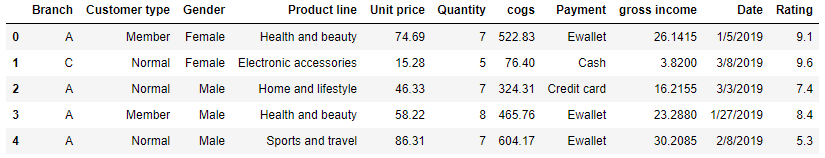
\includegraphics[width=0.9\textwidth]{seg00}
  \caption{Feature Selektion}
  \label{fig:fs00}
\end{figure}

Nach der Bereinigung um irrelevante Features wird, anhand der oftmals aus dem operativen Sektor des CRM stammenden Anfragen, die Grundlage für das Clustering bestimmt.
In diesem Anwendungsbeispiel wird folgende Fragestellung untersucht:

\begin{center}
  \textbf{Gibt es Kundengruppen mit signifikant unterschiedlicher Zufriedenheit?}
\end{center}

Für diese Fragestellung werden die features \textquote{gross income} und \textquote{Date} entfernt, da \textquote{gross income} für den Kunden nicht relevant ist und und \textquote{Date} das Beispiel unnötig Komplex machen würde. Übrig bleibt ein Schema mit Features, auf die der Kunde Einfluss hat (Abb. \ref{fig:fs01}).

\begin{figure}[ht]
  \centering
  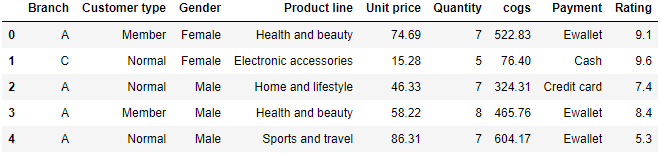
\includegraphics[width=0.9\textwidth]{seg01}
  \caption{Feature Selektion für die Fragestellung}
  \label{fig:fs01}
\end{figure}

Nach der Formulierung der Untersuchungsgrundlage können die Daten weiter um irrelevante Features bereinigt werden.
Daher wird \textquote{gross income} aufgrund fehlender Relevanz entfernt und das Feature \textquote{Date} im Zuge geringerer Komplexität ebenfalls im weiteren Verlauf nicht berücksichtigt.
Damit liegt ein weiter eingegrenztes Schema vor (Abb. \ref{fig:numfeat}).
Unter den Features befinden sich fünf kategorielle Features, von denen zwei binäre Klassen und drei mehrere Klassen besitzen (Abb. \ref{fig:numfeat}).

\begin{figure}[ht]
  \centering
  \begin{tabular}{l | l}
    Feature & Anzahl Ausprägungen\\
    \hline
    Branch & $3$\\
    Customer Type & $2$\\
    Gender & $2$\\
    Product Line & $6$\\
    Payment & $3$
  \end{tabular}
  \caption{Anzahl Ausprägungen in den kategoriellen Features}
  \label{fig:numfeat}
\end{figure}

Für ein Clustering können die kategoriellen Features in numerische Daten transformiert werden.
Durch die anschließende Verwendung eines \textquote{MinMaxScaler} liegt anschließend ein Dataframe gemäß Abbildung \ref{fig:seg02} vor.

\begin{figure}[ht]
  \centering
  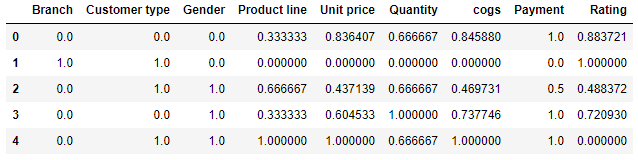
\includegraphics[width=0.9\textwidth]{seg02}
  \caption{Transformierte Daten}
  \label{fig:seg02}
\end{figure}

Für die Wahl der Anzahl an Clustern kann die Elbow-Methode verwendet werden, die auf vier Cluster schließen lässt (Abb. \ref{fig:seg03}).

\begin{figure}[ht]
  \centering
  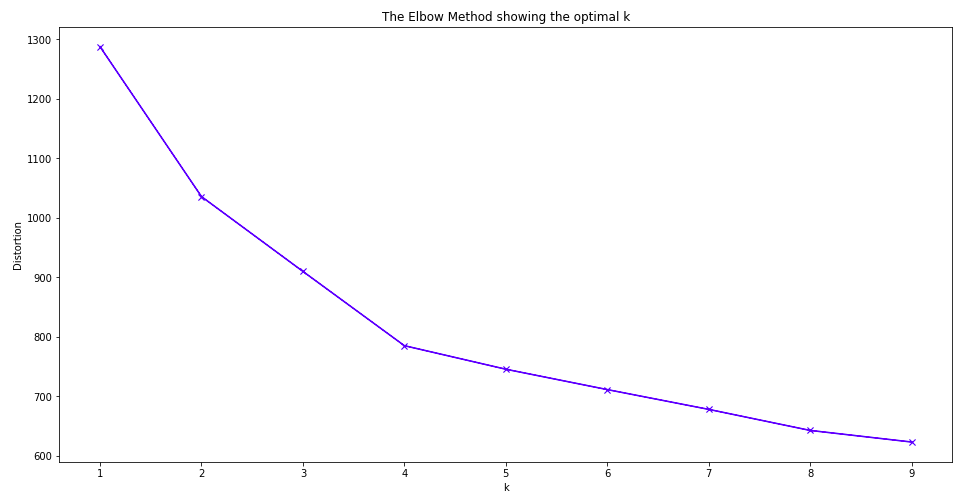
\includegraphics[width=0.9\textwidth]{seg03}
  \caption{Elbow-Methode}
  \label{fig:seg03}
\end{figure}

Aus der Analyse der Ratings innerhalb der Cluster ergeben sich die Zentren aus Abbildung \ref{fig:clusrating}.

\begin{figure}[H]
  \centering
  \begin{tabular}{l | l}
    Cluster & Rating\\
    \hline
    1 & $0.4901021711366539$\\
    2 & $0.5031531531531531$\\
    3 & $0.49$\\
    4 & $0.49840277777777775$
  \end{tabular}
  \caption{Rating Höhe der Cluster}
  \label{fig:clusrating}
\end{figure}

Da die Daten MinMax skaliert sind, bedeutet ein Wert nahe $0.5$, dass der Wert in etwa im Durchschnitt liegt.
Damit kann durch die Auswahl an Features keine Bewertung bezüglich des Ratings abgeleitet werden.

Für die Umsetzung im betrieblichen Kontext bietet es sich an, ein solches Clustering in Business Intelligence Systeme einzubauen, indem man zum Beispiel beliebig Features und Anzahl Cluster auswählen kann und dafür dynamisch den Elbow-Graphen und die Clusterzentren angezeigt bekommt, um so passende Kundensegmentierungen für einzelne Anwendungsfälle der operativen CRM zu erstellen.

\clearpage
\section{Fazit}
\label{sec:fazit}
Die Kundennähe konnte als ein entscheidender Wettbewerbsfaktor gezeigt werden. Erreichen lässt sie sich durch die Analyse der Kundendaten über Methoden der Customer Analytics in Verbindung mit dem CRM. Dabei zeigen sich für Unternehmen je nach Geschäftsmodell unterschiedliche Schwerpunkte und Herausforderungen auf.
Ferner stellt die Auswahl der Features aus Daten eine Herausforderungen dar, die je nach Unternehmensziel stark variieren kann, bietet dabei aber gleichzeitig Möglichkeiten für ein Business Intelligence System.

Die analytische Annäherung über Methoden wie dem Data Mining wird insbesondere bei großen Datenmengen bedeutsam.
Durch eine Segmentierung, ähnlich der des gezeigten Anwendungsbeispiels, kann durch die Berücksichtigung von Kundeninteressen und -eigenschaften eine effizientere Interaktion ermöglicht werden.
Dies kann Kosten des Kundenkontaktes verringern und gleichzeitig durch die verbesserte Ansprache zu einem größeren Unternehmenserfolg führen.

Die Customer Analytics ist für Unternehmen von hoher Relevanz.
Sie bedingt Umstrukturierungen und Veränderungen der Unternehmensstrategien, die langfristig den Bestand und Erfolg des Unternehmens sichern.
Damit ist die Customer Analytics ein unverzichtbarer Teil der Business Intelligence.

% appendix
\clearpage
% \section{Anhang}
\label{sec:anhang}

% \clearpage
% \begin{figure}[H]
%   \caption{Eventlog Analyse Simulation}
%   \label{code:simsensor}
%   \inputminted{python}{res/sim1k-sprt.py}
% \end{figure}

% bib
\clearpage
\printbibliography

\end{document}
